\documentclass[11pt]{article}
\usepackage{amsmath, amssymb, amsthm}
\usepackage[retainorgcmds]{IEEEtrantools}

\usepackage{marginnote}
\usepackage{endnotes}

\usepackage{tikz}
\usetikzlibrary{intersections}
\usetikzlibrary{calc}

\usepackage{fancyhdr}

%Listings stuff
\usepackage{listings}
\usepackage{lstautogobble}
\usepackage{color}

\definecolor{grey}{rgb}{0.5,0.5,0.5}
\lstset{
basicstyle={\small\ttfamily},
tabsize=3,
numbers=left,
numbersep=5pt,
numberstyle=\tiny\color{grey},
stepnumber=2,
breaklines=true
}

%Properly formatted differential 'd'
\newcommand{\ud}{\, \mathrm{d}}

%Format stuff
\pagestyle{fancy}
\headheight 35pt

%Header info
\chead{\Large \textbf{Vectors}}
\lhead{}
\rhead{}

\begin{document}
\section{Basics}
	Definition: A vector $\vec{x}$ is defined as a collection of $n$ ordered numbers $(x_1, x_2,\ldots ,x_n)$.
	
	Basic properties:
	\begin{itemize}
		\item $c(\vec{x} + \vec{y}) = c\vec{x} + c\vec{y}$
		\item $(\vec{x} + \vec{y}) + \vec{z} = \vec{x} + (\vec{y} + \vec{z})$
		\item $(a+b)\vec{x} = a\vec{x} + b\vec{x}$
	\end{itemize}
	
	Other concepts/terms:\marginnote{What is a zero vector?}
	\begin{itemize}
		\item Zero vector: $\vec{0} = (0, 0,\ldots , 0) \text{ and } \vec{x} + \vec{0} = \vec{x} \ \forall \vec{x}$
		\item The \textbf{linear combination} of vectors $\vec{x_1}, \ldots , \vec{x_k} \text{ is } c_1\vec{x_1} + c_2\vec{x_2} + \ldots + c_k\vec{x_k}$ for any real constants.
		\item $\mathbb{R}^n$ represents the set of all real vectors of size $n$.\marginnote{Linear combination?}
		\item Vector Basis: the set of all vectors of size $n$ such that any vector in $\mathbb{R}^n$ can be expressed as a linear combination of the set. The \textbf{standard basis} is $\vec{i}, \vec{j}, \text{ and } \vec{k}$. These vectors are expressed as $\mathbf{\vec{e_k}} = (0, 0, \ldots , 1, 0, \ldots ,0)$, where the lone 1 is at position $k$.\marginnote{Standard basis?}
		\item Unit vector: $\vec{u}=\dfrac{\vec{x}}{|\vec{x}|}$; $\vec{u} = 1$.
		\item Vector distance: $|\vec{x} - \vec{y}|$.
		\item \textbf{Triangle Inequality}: $|\vec{x} + \vec{y}| \leq |\vec{x}| + |\vec{y}|$
	\end{itemize}
	
	\marginnote{Geometric vector add. and sub.?}Geometric representation of vector addition and subtraction (parallelogram method):
	\begin{center}
		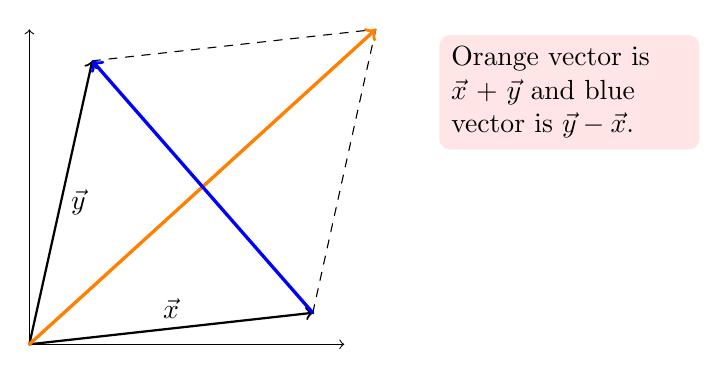
\begin{tikzpicture}
			[scale=4,line cap=round,
			%Styles
			axes/.style=,
			important line/.style={very thick},
			information text/.style={rounded corners,fill=red!10,inner sep=1ex},
			dot/.style={circle,inner sep=1pt,fill,label={#1},name=#1}			
			]
			
			%Colors
			\colorlet{anglecolor}{green!50!black}	%angle arcs/lines
			
			%The graphic
			\begin{scope}[axes]
				\draw[->] (0,0) -- (0,1);
				\draw[->] (0,0) -- (1,0);
			\end{scope}
			
			\draw[->,thick] (0,0) -- node[above] {$\vec{x}$} (.9, .1);
			\draw[->,thick] (0,0) -- node[right] {$\vec{y}$} (.2, .9);
			
			\draw[dashed] (.9,.1) -- (1.1,1);
			\draw[dashed] (.2,.9) -- (1.1,1);
			
			\path[name path=rleg] (.9,.1) -- (1.1,1);
			\path[name path=tleg] (.2,.9) -- (1.1,1);
			
			\draw[->,very thick,orange] (0,0) -- (1.1,1);
			\draw[->,very thick,blue] (.9,.1) -- (.2,.9);
			
			\draw[xshift=1.3cm](0,.8)
				node[right,text width=3cm,information text]
				{
					Orange vector is $\vec{x} + \vec{y}$ and blue vector is $\vec{y} - \vec{x}$.
				};
		\end{tikzpicture}
		\end{center}
		
\section{Points}
	$\mathbb{R}^2 \text{ and } \mathbb{R}^3$ can be used to define points on a plane and in space, respectively.\marginnote{Spherical coordinates?}
	\begin{center}
	\marginnote{Generic magnitude expression?}
	\begin{tikzpicture}
		[scale=2,line cap=round,
		%Styles
		axes/.style=,
		important line/.style={very thick},
		information text/.style={rounded corners,fill=red!10,inner sep=1ex},
		dot/.style={circle,inner sep=1pt,fill,label={#1},name=#1}			
		]
		
		%Colors
		\colorlet{anglecolor}{green!50!black}	%angle arcs/lines
		
		%The graphic
		%\draw[help lines,step=0.5cm,loosely dashed] (-.4,-.4) grid (1.4,1.4);
		
		\begin{scope}[axes]
			\draw[->] (-.2,0) -- (1.5,0) node[right] {$x$} coordinate(x axis);
			\draw[->] (0,-.2) -- (0,1.5) node[above] {$y$} coordinate(y axis);
		\end{scope}
		
		\draw[->,thick,orange] (0,0) -- node[left=3pt] {$\vec{r}$} (1.2,1.2);
		\node [dot=P] at (1,1) {};
		\filldraw[fill=green!20,draw=anglecolor] (0,0) -- node[right=3pt,above,black] {$\theta$}(3mm,0pt) arc (0:45:3mm);
		
		\draw[xshift=1.8cm] (0,.8)
			node[right,text width=5cm,information text]
			{
				\begin{IEEEeqnarray}{rCl}
					\vec{OP} & = & (x_1, x_2)\\
					r & = & \sqrt{x_1^2 + x_2^2}\\
					x_1 & = & r\cos\theta\\
					x_2 & = & r\sin\theta
				\end{IEEEeqnarray}
			};
		
	\end{tikzpicture}
	\marginnote{Convert spherical coord. $\rightarrow$ Cart.?}
	\begin{tikzpicture}
		[scale=3,line cap=round,
		%Styles
		axes/.style=,
		important line/.style={very thick},
		information text/.style={rounded corners,fill=red!10,inner sep=1ex},
		dot/.style={circle,inner sep=1pt,fill,label={#1},name=#1}			
		]
		
		%Colors
		\colorlet{anglecolor}{green!50!black}	%angle arcs/lines
		
		%The graphic
		\begin{scope}[axes]
			\draw[<-] (-.5,-.5) node[right,below] {$x$} coordinate(x axis) -- (0,0);
			\draw[->] (0,0) -- (.7,0) node[right,below] {$y$} coordinate(y axis);
			\draw[->] (0,0) -- (0,.7) node[right,above] {$z$} coordinate(z axis);
		\end{scope}
		
		\draw[->,thick,orange] (0,0) -- node[above=3pt] {$\vec{r}$} (.6,.4);
		\node [dot=P] at (.6,.4) {};
		
		\filldraw[fill=green!20,draw=anglecolor] (0,0) -- (1.5mm,1mm) arc (15:120:1mm) node[above=5pt,right=2pt,black,font=\small] {$\phi$};
		
		\path [name path=zint] (-.25,-.25) -- (1,-.25);
		\path [name path=dropdown] (.6,.4) -- (.6, -1);
		\draw [name intersections={of=zint and dropdown, by=t}]
			[dashed] (.6,.4) -- (t);
		\draw [dashed] (-.25,-.25) -- (t);
		\draw[->] (0,0) -- (t);
		
		\path [name path=oq] (0,0) -- (t);
		\path [name path=phicircle] (0,0) circle (1mm);
		
		\filldraw [name intersections={of=oq and phicircle, by=u}]
			[fill=green!20,draw=anglecolor] (0,0) -- (u) arc (-20:-135:1mm) node[right=3pt,below,black,font=\small] {$\theta$};
			
		\draw[xshift=1cm]
			node[right,text width=6.5cm,information text]
			{
				The \textbf{spherical coordinates} (Figure \ref{fig:spherical}) defined by $(r,\phi,\theta)$, where $\theta$ is \textit{azimuth} along the equator and $\phi$ is \textit{inclination} from the meridian, can be converted to Cartesian coordinates.
				\begin{IEEEeqnarray}{rCl}
					r & = & \sqrt{x_1^2+x_2^2+x_3^2}\\
					x_1 & = & r\sin\phi\cos\theta\\
					x_2 & = & r\sin\phi\sin\theta\\
					x_3 & = & r\cos\theta
				\end{IEEEeqnarray}
			};
	
	\end{tikzpicture}
	\end{center}		
	
	\begin{figure}[htb]
		\centering
		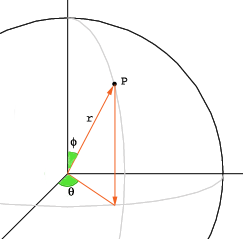
\includegraphics[width=0.4\textwidth]{vectorsfig3.png}
		\caption{Spherical coordinates.}
		\label{fig:spherical}
	\end{figure}
	
\section{Lines}
	There are two ways to specify a line with vectors: either as passing through a point in a direction, or as passing through 2 points.
	
	With the former method, given a nonzero vector $\vec{u}$, the line through the origin in the direction of $\vec{u}$ consists of all points whose position vectors are multiples of $\vec{u}$. If we translate all points by a vector $\vec{v}$, we get a generic definition for a line.
	\marginnote{Parametric line equation?}
	\begin{equation}
		l = t\vec{x_0} + \vec{v} \quad \forall \ t \in \mathbb{R} \text{ and } \vec{x_0}\neq 0
	\end{equation}
	
	This is called the \textbf{parametric representation} of a line where $t$ is the \textbf{parameter}.
	
	\begin{center}
		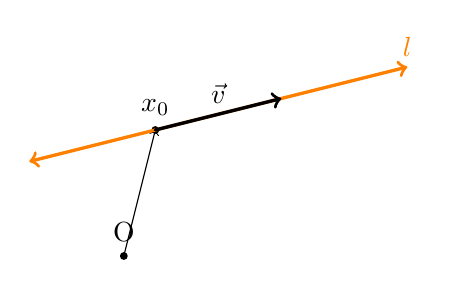
\begin{tikzpicture}
			[scale=4,line cap=round,
			%Styles
			axes/.style=,
			important line/.style={very thick},
			information text/.style={rounded corners,fill=red!10,inner sep=1ex},
			dot/.style={circle,inner sep=1pt,fill,label={#1},name=#1}			
			]
			
			%Colors
			\colorlet{anglecolor}{green!50!black}	%angle arcs/lines
			
			%The graphic
			\node [dot=O] at (0,0) {};
			\node [dot=$x_0$] at (.1,.4) {};
			\draw[->] (0,0) -- (.1, .4);
			
			
			\draw[<->,orange,very thick] (-.3,.3) -- (.9,.6) node[above] {$l$} ;
			\draw[->,very thick] (.1, .4) -- node[above] {$\vec{v}$} (.5,.5);
			
			%\draw[->] (.4,.8) \node[above] {$t\vec{v}$} -- (1,1);
		\end{tikzpicture}
	\end{center}
	
	\marginnote{Equation for line through 2 points?}When given two position vectors $\vec{a} \text{ and } \vec{b}$, it is possible to represent the line passing through both as such:
	
	\begin{IEEEeqnarray}{rCl}
		\vec{x} & = & t(\vec{b}-\vec{a}) + \vec{a}\\
		\vec{x} & = & (1-t)\vec{a} + t\vec{b}
	\end{IEEEeqnarray}
	
	When $t=0, \vec{x} = \vec{a}$ and when $t=1, \vec{x} = \vec{b}$.
	
\section{Planes}
	\marginnote{Equation of plane?}There is a unique plane that will contain any two nonzero vectors. The parametric representation of a plane is as follows:
	\begin{equation}
		\mathbf{x} = \vec{x_0} + s\vec{u} + t\vec{v}
	\end{equation}
	
	$\vec{x_0}$ is the linear shift of the origin. Note that if $\vec{x_0} = 0$, the plane is a linear combination of the vectors $\vec{u}$ and $\vec{v}$. Another condition for the plane is that $\vec{u}$ and $\vec{v}$ must be \textbf{linearly independent}, meaning neither is a scalar multiple of the other.
	
	A characteristic property of planes is that if the points $\mathbf{p}$ and $\mathbf{q}$ are both in the plane, the line that passes through them is entirely in the plane as well.
	
	In general, in the set of vectors $\mathbb{R}^n$ and an $n$-dimensional space, the equation for a $k$-dimensional hyperplane in space is as follows:
	\begin{equation}
		\vec{x}(t_1,\ldots ,t_k) = \vec{x_0} + t_1\vec{u_1} + t_2\vec{u_2} + \ldots + t_k\vec{u_k}
	\end{equation}
	
\section{Dot Products}
	\marginnote{What are dot products?}Definition:
	\begin{equation}
		\vec{x} \cdot \vec{y} = x_1y_1 + x_2y_2 + \ldots + x_ny_n
	\end{equation}
	
	Given this, the equation for $|\vec{x}|$ can be written as
	\begin{equation}
		|\vec{x}| = \sqrt{\vec{x}\cdot\vec{x}}
	\end{equation}
	
	\subsection{Law of Cosines}
		\begin{center}
			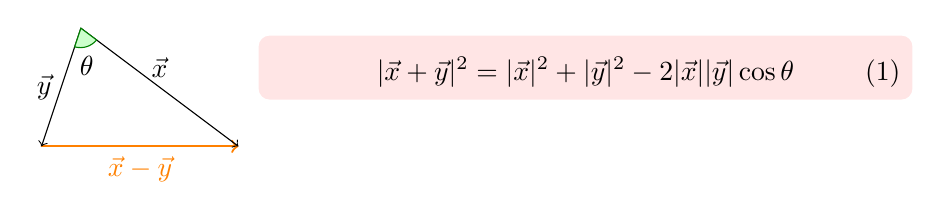
\begin{tikzpicture}
				[scale=.5,line cap=round,
				%Styles
				axes/.style=,
				important line/.style={very thick},
				information text/.style={rounded corners,fill=red!10,inner sep=1ex},
				dot/.style={circle,inner sep=1pt,fill,label={#1},name=#1}			
				]
				
				%Colors
				\colorlet{anglecolor}{green!50!black}	%angle arcs/lines
				
				%The graphic
				\coordinate (a) at (0,0);
				\coordinate (b) at (1,3);
				\coordinate (c) at (5,0);
				
				\draw[->,orange,thick] (a) -- node[below] {$\vec{x} - \vec{y}$} (c);
				\draw[->] (b) -- node[left] {$\vec{y}$} (a);
				\draw[->] (b) -- node[above] {$\vec{x}$} (c);				
				
				\filldraw[fill=green!20,draw=anglecolor] (b) -- ($(b)!5mm!(c)$) to[bend left] node[below,black] {$\theta$} ($(b)!5mm!(a)$) -- cycle;
				
				\draw[xshift=5.5cm] (0,2)
					node[right,text width=8cm,information text]
					{
						\begin{equation}
							|\vec{x} + \vec{y}|^2 = |\vec{x}|^2 + |\vec{y}|^2 - 2|\vec{x}||\vec{y}|\cos\theta
							\label{eqn:law cos}
						\end{equation} 
					};
			\end{tikzpicture}
		\end{center}
		
		From the Law of Cosines (\ref{eqn:law cos}), it is possible to derive a second definition of the cross product.
		\begin{IEEEeqnarray}{rCl}
			|\vec{x} + \vec{y}|^2 & = & |\vec{x}|^2 + |\vec{y}|^2 - 2|\vec{x}||\vec{y}| \\\nonumber
			|\vec{x} + \vec{y}|^2 & = & |\vec{x}|^2 + |\vec{y}|^2 - 2|\vec{x}||\vec{y}|\cos\theta\\
			\vec{x}\cdot\vec{y} & = & |\vec{x}||\vec{y}|\cos\theta\label{eqn:dotp2}
		\end{IEEEeqnarray}
		
		By re-arranging equation \ref{eqn:dotp2}, we get an expression for calculating the angle between two vectors.
		\begin{equation}
			\theta = \arccos\frac{\vec{x}\cdot\vec{y}}{|\vec{x}||\vec{y}|}
		\end{equation}
		
	\subsection{Theorem of Pythagoras}
		\begin{equation}
			\text{If } \vec{x}\cdot\vec{y} = 0, \text{ then } |\vec{x} - \vec{y}| = |\vec{x}|^2 + |\vec{y}|^2
		\end{equation}
		
		This is essentially Pythagorean's Theorem applied to vectors. Two vectors are called \textbf{orthogonal} to each other if their dot product is 0.
		
	\subsection{Cauchy-Schwartz Inequality}
		\marginnote{Cauchy-Schwartz?}\begin{equation}
			|\vec{x}\cdot\vec{y}| = |\vec{x}||\vec{y}||\cos\theta|\leq |\vec{x}||\vec{y}|
		\end{equation}
		
	\subsection{Projections}
		\marginnote{Projections?}The \textbf{projection} of one vector onto another is the component of the first that is in the same direction as the second. Given a unit vector $\vec{n}$, the projection of $\vec{x}$ can be expressed as $\Pr_{\vec{n}}(\vec{x}) = c\vec{n}$.
		
		\begin{center}
			\begin{tikzpicture}
				[scale=1,line cap=round,
				%Styles
				axes/.style=,
				important line/.style={very thick},
				information text/.style={rounded corners,fill=red!10,inner sep=1ex},
				dot/.style={circle,inner sep=1pt,fill,label={#1},name=#1}			
				]
				
				%Colors
				\colorlet{anglecolor}{green!50!black}	%angle arcs/lines
				
				%The graphic
				\coordinate (a) at (0,0);
				\coordinate (b) at (3,0);
				\coordinate (c) at (3,2);
				
				\draw[->,orange] (a) -- node[below=10pt] {$Pr_{\vec{n}}(\vec{x})$} (b);
				\draw[->] (a) -- node[left] {$\vec{x}$} (c);
				\draw ($(b)!3mm!(a)$) -- +(0,3mm) -- ($(b)!3mm!(c)$);			
				
				\draw[dashed,black!30] (c) -- (b);
				\draw[->,very thick] (a) -- node[below] {$\vec{n}$} (1,0);
				
				\draw[xshift=3.5cm] (0,1)
					node[right,text width=6cm,information text]
					{
						\begin{IEEEeqnarray}{rCl}
							(\vec{x} - c\vec{x})\cdot\vec{n} & = & 0\\
							\nonumber \vec{n}\cdot\vec{n} & = & 1\\
							c & = & \vec{x}\cdot\vec{n}\\
							Pr_{\vec{n}}(\vec{x}) & = & (\vec{x}\cdot\vec{n})\vec{n}\label{eqn:norm pr}
						\end{IEEEeqnarray}
					};
			\end{tikzpicture}
		\end{center}
		
		The vector $\vec{n}$ in equation \ref{eqn:norm pr} is called a \textbf{normalization} because it is a reduction of a vector of arbitrary length to a unit vector in the same direction.
		
\section{Euclidean Geometry}
	It is possible to use the dot product to determine the equations of lines and planes and to extrapolate these equations to higher dimensions.
	
	\subsection{Equations of Lines and Planes}
		Given that $\vec{x_0}$ is a fixed point on a line in $\mathbb{R}^2$ or a plane in $\mathbb{R}^3$ and $\vec{n}$ is perpendicular to the line or plane, every point $\vec{x}$ must satisfy the following equation, given $\vec{x_0}$ is any point on the plane.
		\marginnote{Dot product form of lines and planes?}\begin{equation}
			\vec{n}\cdot(\vec{x}-\vec{x_0}) = 0
			\label{eqn:plane}
		\end{equation}
		
		Because $\vec{n}$ is a unit vector and $\vec{x_0}$ is a fixed point, a plane or line can also be described with the following equation.
		\begin{equation}
			\vec{n}\cdot\vec{x} - c = 0;
		\end{equation}
		
		\begin{center}
			\begin{tikzpicture}
				[scale=1,line cap=round,
				%Styles
				axes/.style=,
				important line/.style={very thick},
				information text/.style={rounded corners,fill=red!10,inner sep=1ex},
				dot/.style={circle,inner sep=1pt,fill,label={#1},name=#1}			
				]
				
				%Colors
				\colorlet{anglecolor}{green!50!black}	%angle arcs/lines
				
				%The graphic
				\coordinate (p) at (0,0);
				\coordinate (a) at (3,3);
				\coordinate (b) at (6,0);
				\coordinate (c) at (3,1);
				\coordinate (d) at (5,1);
				
				\draw[->] (p) node[left] {$P$} -- (a);
				\draw[->] (p) -- (b);
				
				\path [name path=x0] (1,-2)--(c);
				\path [name path=u] (p) -- (b);
				\draw[name intersections={of={x0 and u}, by=i}][orange,thick] (1,-2)-- node[left]{$x_0$} (i);
				\draw[orange,thick,dashed,->] (i)--(c);
				
				\draw[orange,thick,->] (c) -- node[left] {$\vec{n}$} +(0,1);
				\draw[blue,->] (c) -- node[above]{$\vec{x}-\vec{x_0}$} (d);
				\draw[blue,thick,->] (1,-2) -- node[right]{$\vec{x}$} (d);
				\draw ($(c)!2mm!(d)$) -- +(0,2mm) -- +(-2mm,2mm);
				\draw(0,-4.5)
					node[right,text width=10cm,information text]
					{
						\begin{IEEEeqnarray}{rCl}
							\nonumber\vec{x} = (x,y,z);\vec{x_0} & = & (x_0,y_0,z_0);\vec{n} = (a,b,c)\\
							(\vec{x}-\vec{x_0})\cdot\vec{n} & = & 0\\
							(x-x_0)a+(y-y_0)b+(z-z_0)c & = & 0\\
							ax+by+cz & = & ax_0+by_0+cz_0\\
							ax+by+cz & = & d
						\end{IEEEeqnarray}
					};
			\end{tikzpicture}
		\end{center}
		
	\subsection{Distance to a Line or Plane}
		\marginnote{Distance to line or plane?}Given a plane defined by equation \ref{eqn:plane}, the distance from a point $\vec{x_1}$ to $P$ is
		\begin{equation}
			\delta = \vec{n}\cdot(\vec{x_1}-\vec{x_0})
		\end{equation}
		
		\marginnote{Explain the formula}if $\vec{x_1}$ is on the side of $P$ with the tip of $\vec{n}$, and $-\delta$ on the other side. Since $|\vec{n}| = 1$, we can also express the normalized distance equation as follows, where $\theta$ is the angle between $\vec{n}$ and $\vec{x_1}-\vec{x_0}$.
		\begin{equation}
			\delta = |\vec{x_1}-\vec{x_0}|\cos\theta
		\end{equation}
		
\section{Cross Products}
	\begin{equation}
		\vec{x}\times\vec{y} = (x_2y_3-x_3y_2)\hat{i}+(x_3y_1-x_1y_3)\hat{j}+(x_1y_2-x_2y_1)\hat{k}
	\end{equation}
	\marginnote{Cross product calculation?}\begin{equation}
		\vec{x}\times\vec{y} = det
		\begin{vmatrix}
			\hat{i} & \hat{j} & \hat{k}\\
			x_1 & x_2 & x_3\\
			y_1 & y_2 & y_3
		\end{vmatrix}
	\end{equation}
	\marginnote{Cross product magnitude?}\begin{equation}
		|\vec{x}\times\vec{y}| = xy\sin\theta
	\end{equation}
	
	\subsection{Scalar Triple Product}
		\marginnote{Scalar triple product?}The scalar triple product of three vectors $\vec{u}, \vec{v}, \text{ and }\vec{w}$ is $\vec{u}\cdot(\vec{v}\times\vec{w})$. The scalar triple product of three vectors is equal to the volume of the \textbf{parallelepiped} defined by the three vectors (space bounded by three pairs of congruent parallelograms). 
		
		\marginnote{Flux?}The generic equation for flux across a parallelogram is also a scalar triple product. Given $\vec{p},\vec{q}$ are adjacent edges of a parallelogram $P$, the flux $\Phi$ is defined as follows.
		\begin{equation}
			\Phi = A(P)\vec{n}\cdot\vec{v} = |\vec{p}\times\vec{q}|\frac{\vec{p}\times\vec{q}}{|\vec{p}\times\vec{q}|}\cdot\vec{v} = \vec{v}\cdot(\vec{p}\times\vec{q})
		\end{equation}
		
\section*{Important Concepts}
	\subsection*{Vectors, Lines, and Planes}
		\begin{itemize}
			\item Spherical coordinates: $(r,\phi,\theta)$, $\phi$: inclination, $\theta$: azimuth.
			\item \begin{IEEEeqnarray*}{rCl}
					x_1 & = & r\sin\phi\cos\theta\\
					x_2 & = & r\sin\phi\sin\theta\\
					x_3 & = & r\cos\phi
				\end{IEEEeqnarray*}
			\item \begin{IEEEeqnarray*}{rCl}
				\vec{x}(t) & = & \vec{x_0} + t\vec{v}\\
				\vec{x}(t) & = & t(\vec{b}-\vec{a}) + \vec{a}
				\end{IEEEeqnarray*}
			\item $\mathbf{x} = \vec{x_0}+s\vec{u}+t\vec{v}$
		\end{itemize}
		
	\subsection*{Dot Products}
		\begin{itemize}
			\item $\vec{x}\cdot\vec{y} = x_1y_1 + x_2y_2 +\ldots + x_ny_n$
			\item $\vec{x}\cdot\vec{y} = xy\cos\theta$
			\item $|\vec{x}|^2 = \vec{x}\cdot\vec{x}$
		\end{itemize}
		
		\subsubsection*{Projections}
			\begin{itemize}
				\item $\vec{x}_{\vec{n}} = (\vec{x}\cdot\vec{n})\vec{n}$
				\item Component of vector in direction of another.
			\end{itemize}
			
		\subsubsection*{Lines and Planes Revisited}
			\begin{itemize}
				\item $\vec{n}\cdot(\vec{x}-\vec{x_0}) = 0, \vec{x_0}$ is point on plane or line, $\vec{n}$ is normal to plane or line.
				\item $\delta = \vec{n}\cdot(\vec{x_1}-\vec{x_0})$ gives distance from a point to plane or line ($\vec{n}$ is unit vector).
			\end{itemize}
			
	\subsection*{Cross Products}
		\begin{itemize}
			\item $\vec{x}\times\vec{y} = (x_2y_3-x_3y_2)\hat{i}+(x_3y_1-x_1y_3)\hat{j}+(x_1y_2-x_2y_1)\hat{k}$
			\item $\vec{x}\times\vec{y} = det
		\begin{vmatrix}
			\hat{i} & \hat{j} & \hat{k}\\
			x_1 & x_2 & x_3\\
			y_1 & y_2 & y_3
		\end{vmatrix}$
			\item $|\vec{x}\times\vec{y}| = xy\sin\theta$
		\end{itemize}
		
		\subsubsection*{Scalar Triple Product}
			\begin{itemize}
				\item $\vec{u}\cdot(\vec{v}\times\vec{w})$
				\item Gives the volume of a parallelepiped bound by three vectors.
				\item Flux: \[\Phi = A(P)\vec{n}\cdot\vec{v} = |\vec{p}\times\vec{q}|\frac{\vec{p}\times\vec{q}}{|\vec{p}\times\vec{q}|}\cdot\vec{v} = \vec{v}\cdot(\vec{p}\times\vec{q})\]
			\end{itemize}
%		\def\enotesize{\normalsize}
%		\theendnotes
\end{document}